\documentclass[working, oneside]{inputs/tuftebook}
\usepackage[utf8]{inputenc}
\usepackage[T1]{fontenc}
\usepackage{textcomp}

\usepackage{url}

\usepackage[
    sorting=nyt,
    style=alphabetic
]{biblatex}
\addbibresource{bibliography.bib}

\usepackage{hyperref}
\hypersetup{
    colorlinks,
    linkcolor={black},
    citecolor={black},
    urlcolor={blue!80!black}
}
\usepackage[noabbrev]{cleveref}

% Adds Bibliography, ... to Table of Contents
\usepackage[nottoc]{tocbibind}

\usepackage{graphicx}
\usepackage{float}
\usepackage[usenames,dvipsnames,svgnames]{xcolor}

% \usepackage{cmbright}

\usepackage{amsmath, amsfonts, mathtools, amsthm, amssymb}
\usepackage{mathrsfs}
\usepackage{cancel}

\newcommand\N{\ensuremath{\mathbb{N}}}
\newcommand\R{\ensuremath{\mathbb{R}}}
\newcommand\Z{\ensuremath{\mathbb{Z}}}
\renewcommand\O{\ensuremath{\emptyset}}
\newcommand\Q{\ensuremath{\mathbb{Q}}}
\newcommand\C{\ensuremath{\mathbb{C}}}
\let\implies\Rightarrow
\let\impliedby\Leftarrow
\let\iff\Leftrightarrow
\let\epsilon\varepsilon

\usepackage{tikz}
\usepackage{tikz-cd}

% theorems
\usepackage{thmtools}
\usepackage{thm-restate}
\usepackage[framemethod=TikZ]{mdframed}
\mdfsetup{skipabove=1em,skipbelow=0em, innertopmargin=12pt, innerbottommargin=8pt}

\theoremstyle{definition}

\makeatletter

\declaretheoremstyle[headfont=\bfseries\sffamily, bodyfont=\normalfont, mdframed={ nobreak } ]{thmgreenbox}
\declaretheoremstyle[headfont=\bfseries\sffamily, bodyfont=\normalfont, mdframed={ nobreak } ]{thmredbox}
\declaretheoremstyle[headfont=\bfseries\sffamily, bodyfont=\normalfont]{thmbluebox}
\declaretheoremstyle[headfont=\bfseries\sffamily, bodyfont=\normalfont]{thmblueline}
\declaretheoremstyle[headfont=\bfseries\sffamily, bodyfont=\normalfont, numbered=no, mdframed={ rightline=false, topline=false, bottomline=false, }, qed=\qedsymbol ]{thmproofbox}
\declaretheoremstyle[headfont=\bfseries\sffamily, bodyfont=\normalfont, numbered=no, mdframed={ nobreak, rightline=false, topline=false, bottomline=false } ]{thmexplanationbox}

\declaretheoremstyle[headfont=\bfseries\sffamily, bodyfont=\normalfont, numbered=no, mdframed={ nobreak, rightline=false, topline=false, bottomline=false } ]{thmexplanationbox}


\declaretheorem[numberwithin=chapter, style=thmgreenbox, name=Definition]{definition}
\declaretheorem[sibling=definition, style=thmredbox, name=Corollary]{corollary}
\declaretheorem[sibling=definition, style=thmredbox, name=Proposition]{prop}
\declaretheorem[sibling=definition, style=thmredbox, name=Theorem]{theorem}
\declaretheorem[sibling=definition, style=thmredbox, name=Lemma]{lemma}
\declaretheorem[sibling=definition, style=thmbluebox,  name=Example]{eg}
\declaretheorem[sibling=definition, style=thmbluebox,  name=Nonexample]{noneg}
\declaretheorem[sibling=definition, style=thmblueline, name=Remark]{remark}




\declaretheorem[numbered=no, style=thmexplanationbox, name=Proof]{explanation}
\declaretheorem[numbered=no, style=thmproofbox, name=Proof]{replacementproof}
\declaretheorem[style=thmbluebox,  numbered=no, name=Exercise]{ex}
\declaretheorem[style=thmblueline, numbered=no, name=Note]{note}

% \renewenvironment{proof}[1][\proofname]{\begin{replacementproof}}{\end{replacementproof}}

% \AtEndEnvironment{eg}{\null\hfill$\diamond$}%

\newtheorem*{uovt}{UOVT}
\newtheorem*{notation}{Notation}
\newtheorem*{previouslyseen}{As previously seen}
\newtheorem*{problem}{Problem}
\newtheorem*{observe}{Observe}
\newtheorem*{property}{Property}
\newtheorem*{intuition}{Intuition}


\declaretheoremstyle[
    headfont=\bfseries\sffamily\color{RawSienna!70!black}, bodyfont=\normalfont,
    mdframed={
        linewidth=2pt,
        rightline=false, topline=false, bottomline=false,
        linecolor=RawSienna, backgroundcolor=RawSienna!5,
    }
]{todo}
\declaretheorem[numbered=no, style=todo, name=TODO]{TODO}


\usepackage{etoolbox}
\AtEndEnvironment{vb}{\null\hfill$\diamond$}%
\AtEndEnvironment{intermezzo}{\null\hfill$\diamond$}%

% http://tex.stackexchange.com/questions/22119/how-can-i-change-the-spacing-before-theorems-with-amsthm
% \def\thm@space@setup{%
%   \thm@preskip=\parskip \thm@postskip=0pt
% }

\usepackage{xifthen}

\makeatother

% figure support (https://castel.dev/post/lecture-notes-2)
\usepackage{import}
\usepackage{xifthen}
\pdfminorversion=7
\usepackage{pdfpages}
\usepackage{transparent}


\makeatletter
\newif\ifworking
\@ifclasswith{tuftebook}{working}{\workingtrue}{\workingfalse}
\makeatother

\newcommand{\incfig}[2][1]{%
    % \ifworking{\makebox[0pt][c]{\color{gray}{\scriptsize\textsf{#2}}}}\fi%
    \def\svgwidth{#1\textwidth}
    \import{./figures/}{#2.pdf_tex}
}

\newcommand{\fullwidthincfig}[2][0.90]{%
    % \ifworking{\makebox[0pt][l]{\color{gray}{\scriptsize\textsf{#2}}}}\fi%
    \def\svgwidth{#1\paperwidth}
    \import{./figures/}{#2.pdf_tex}
}



\newcommand{\minifig}[2]{%
    \def\svgwidth{#1}%
    \begingroup%
    \setbox0=\hbox{\import{./figures/}{#2.pdf_tex}}%
    \parbox{\wd0}{\box0}\endgroup%
    \hspace*{0.2cm}
}

% %http://tex.stackexchange.com/questions/76273/multiple-pdfs-with-page-group-included-in-a-single-page-warning
\pdfsuppresswarningpagegroup=1

\newcommand\todo[1]{\ifworking {{\color{red}{#1}}} \else {}\fi}
\newcommand\charlotte[1]{\ifworking {{\color{blue}{#1}}} \else {}\fi}

\author{Gilles Castel}



\usepackage{multirow}
\def\block(#1,#2)#3{\multicolumn{#2}{c}{\multirow{#1}{*}{$ #3 $}}}

% \overfullrule=1mm

\newenvironment{myproof}[1][\proofname]{%
  \proof[\rm \bf #1]%
}{\endproof}

\usepackage{pdfpages}

\usepackage{lipsum}
\usepackage{parskip}
\usepackage{titletoc}

\usepackage{cmbright}
\usepackage{bm}
\addbibresource{bibliography.bib}

\begin{document}
% 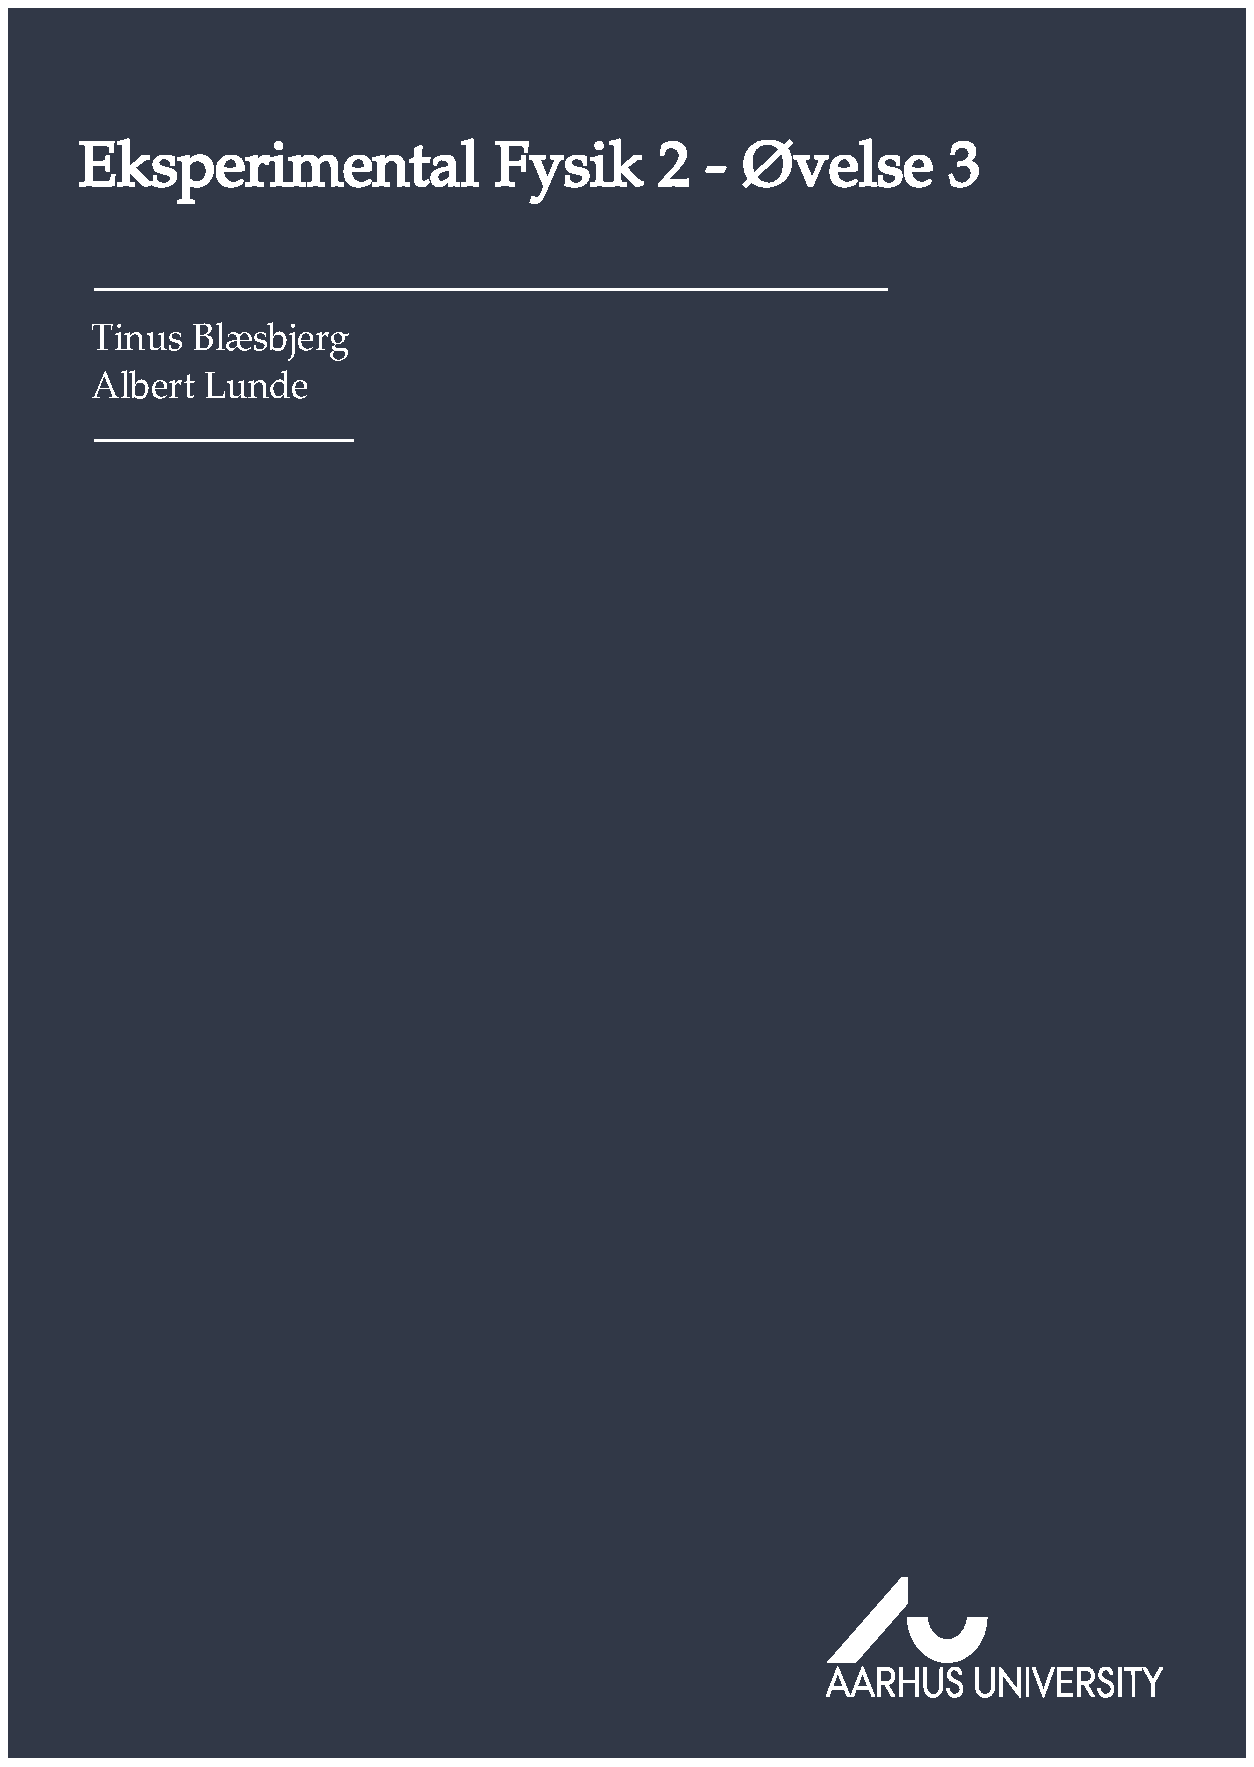
\includepdf[pages=-, fitpaper=true]{inputs/frontmatter.pdf}
\section*{Introduction}
In this experiment we look into the nature of how  electromagnetic waves are emitted and absorbed. Firstly we look at an absorption spectrum from the sun to examine what kind of materials it consists of and then we use Planck's law of black-body radiation to examine the temperature of the sun. Secondly we examine how the absorption of light depends on the concentration of a given substance - in this case green food colouring.
\section*{Theory}
\subsection*{Spectrometer}
We shall first, in short, explain how a spectrometer works and what it is used. A spectrometer is a device that can measure the spectral composition of light. Fig. 1 shows the spectrum of hydrogen. The most common form of spectrometer, which is also what we have used, is a grating spectrometer. A grating spectrometer, separates the light by wavelength with a periodic grate, as illustrated in fig 2. Let us a consider a monochromatic component of light. As it is reflected off the grate it will only create construcive interference at specific angles. This angle is related to the wavelength by the follwing formula called the 'grating equation'
\[
d\left( \sin \theta_i - \sin \theta_m \right) = \lambda m \quad \text{where}\quad  m = \pm 0, \pm 1, \pm 2 \ldots
.\] 
\subsection*{Absorbtion}
When electromagnetic waves travel in a media some of the electromagnetic energy in the wave is transformed to internal energy in the media. E.g the intensity of light decreases when it passes through a media. The relationship between the ingoing intensity and outgoing intensity is called absorbance and given by:
\[
A = log_{10}(\frac{I_{In}}{I_{Out}})
\]
Where A is the absorbance, $I_{In}$ is the ingoing intensity and $I_{Out}$ is the outgoing intensity. The fraction in the logarithm is equal to $\frac{1}{T}$, where T is the transmittance. The use of an logarithmic scale allows for a more compromised graph and also makes it easier to spot how many the percentile difference between two points. \\
There also exists another equation for absorbance which is called the Lambert-Beer law. The amount of light that gets absorbed depends on what media the light is travelling through and how far it needs to travel in the media. The relation is:
\[
A = \epsilon c l
\]  
Where $\epsilon$ it the absorptivity of the material, c is the concentration of the media and l is the length the light has to travel in the media. This relation is very useful because it can be used to display a linear relationship between the absorbance and the concentration of a liquid.
\\
Different materials absorbs differently in the visible spectrum e.g the sea is blue because it absorbs least light in the blue part of the spectrum. Sending light through a material can then be used to determine what the material is.
\subsection*{Emission}
All elements have different spectra. These are to the specific energy levels where they are able to absorb light (different wavelengths of light have different energy levels). These energy levels are the possible excited states that the elements electronic structure can be in. An element emits light, when its electron structure descends in energy. The energy of light emitted is then equal to the magnitude of the descent. As a consequence an element can only emit light with specific energies.
\section*{Experimental set-up}
\subsubsection*{Emission}
The spectrometer given for the experiment could be used to measure the emission spectrum of any given light source. It was plugged into the computer where we could take a background measurement and subtract it from the actual measurement. An optical fibre cable could then be connected to the spectrometer to increase the range of the spectrometer. This was then used to measure the emission spectrum of the sun.
\subsubsection*{Absorption}
For this part of the exercise a lamp module tool was connected to the spectrometer. This tool had a small  empty space where one could place a container with a liquid. The lamp module would then send electromagnetic waves through the sample which could  be detected by the spectrometer on the other side of the sample. Depending on the concentration and substance different amounts of intensity would receive the spectrometer. For our experiment we had a container with water placed in the empty space of the lamp tool. Between each measurement we would then put a droplet of green fruit colouring in container using a plastic strip.  
\section*{Results}
\subsection*{Absorption}
From the theory section we knew that if the absorbance could be measured it could be related to the concentration of the substance by Lambert-Beer's law. The spectrometer connected with the lamb module tool could report what the absorbance of the sample was. Since we took a reference measurement of the absorption spectrum of water, all the measurement made became a relative absorbance with respect to water. This meant that the length of the container could be neglected in the calculations. Our goal was then to see how the the absorbance of the sample depended on the amount of fruit colouring drops in the sample. Since the absorbance is linearly dependent on the concentration of the solute we would expect a linear increase in the absorbance each time we increase the concentration by adding droplets. The hard part is that we cannot exactly know if the concentration increases linearly with the amounts of drops we put in the solution. We would need to have a bunch of different information we don't have. Eg. the molar mass, the volume of a droplet and either the density or the mass of the green food colouring. This will be discussed further in the discussion section. \\
\begin{marginfigure}
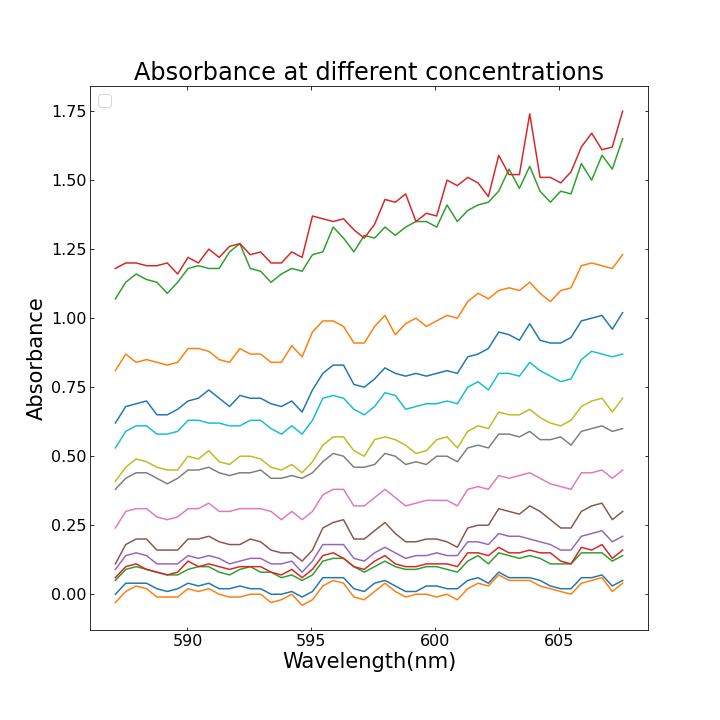
\includegraphics[scale=0.28]{absorbance.png}
\caption{This is only a small sample from the whole dataset. The different colors represent different solutions. It can be seen that when the concentration increases then the absorbance increases as well}
\end{marginfigure}
Assuming the relationship between the absorbance and the amount of droplets was linear, a fit was made. Though it seems to appear that function is only linear in the beginning. The function $y = ax + b$ yielded coefficients of:
\begin{center}
a = 0.091 $\pm$ 0.0084 
\smallskip

b = -0.289 $\pm$ 0.071.
\end{center}
Though by just looking at the graph the fit seems more polynomial and appears that the absorbance increases more rapidly with the latter drops, so a polynomial fit was also made. The function $y = ax^2 + bx +c$ yielded coefficients of:
\begin{center}
a = 0.0078 $\pm$ 0.0007,
\smallskip
 
b = -0.025 $\pm$ 0.011,
\smallskip 

c = 0.021 $\pm$ 0.037
\end{center}
\begin{marginfigure}
\centering
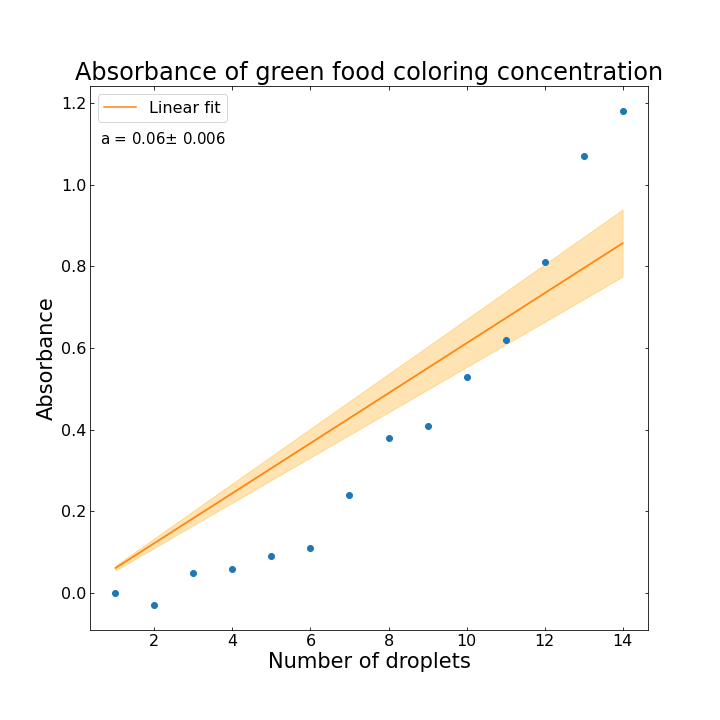
\includegraphics[scale=0.28]{droplets.png}
\caption{A plot showing how the absorbance of a solution of water and green food colouring depends on the amount of green food colouring droplets in the solution. A linear fit and a polynomial fit was made.\\ 
\textbf{LinearFit($ax+b$):} a = 0.091 $\pm$ 0.0084, b = -0.289 $\pm$ 0.071. \\
\textbf{PolynomialFit($ax^2 + bx +c$)}: a = 0.0078 $\pm$ 0.0007, b = -0.025 $\pm$ 0.011, c = 0.021 $\pm$ 0.037}
\end{marginfigure}
I can be seen that the first and second point on the graph is very close to the absorbance spectrum of water and the second point even has an absorbance below 0.0, which just indicates that the these two drops did not make a remarkable difference. This is not to unnatural since the natural fluctuation in the measurement of the spectrum makes it possible to actually measure an absorbance that is lower.


\section*{Discussion}
\subsection*{Absorption}
This turned out to be quite a bad experiment for an obvious reason. We could not get our hands on a pipette so we had to use some kind of plastic strip which made it hard to control the amount of food colouring we put in the container. This can also be seen in the data where it is quite obvious that change in absorbance between two measurements are larger in the latter measurements than in the earlier measurements. This inconsistency would properly be resolved by using a pipette.  \\

In this experiment we also increased the concentration of the solution by adding more droplets but can we even say that the concentration increases linearly with the amount of droplets? To know this we would need to know how the concentration changes when adding a droplet. The concentration is given by:
\begin{center}
$c = \frac{n}{V}$
\end{center}
Where c is the concentration in $\frac{mol}{L}$, n is the amount of solute in the solution given in mol and V is volume of the mixture in L. One can rewrite the equation to:
\begin{center}
$c = \frac{m}{MV}$
\end{center}
Where m is the mass in g and M is the molar mass in $\frac{g}{mol}$. It is properly not a bad approximation to assume that a droplet of the food colouring contributes with the same volume and same mass every time. Since the volume of the droplet is very small compared to the volume of the water we can approximate:
\begin{center}
$c=\frac{mx}{M\cdot(V_{water}+V_{droplet}x)}$
\smallskip

When $V_{droplet}$ << $V_{water}$: \:  $ c\approx \frac{mx}{M\cdot V_{water}}$
\end{center}

Where x is number of droplets. This shows a linear increase is a good approximation. Since the molar mass actually is accessible on the internet one could also calculate the absorptivity if the density of the of the food colouring could be determined. \\

\subsubsection*{Linear fit}
The a-coefficient is actually quite precise and has a relative small error compared to the b-coefficient which has quite a large error. Even though the a coefficient has a small error it is hard to argue from our data that there exists a linear relationship between the absorbance and the amount of droplets. Just by looking at the graph it does not look linear and this very much caused by the inconsistency between the early and late measurements. If this consistency had existed we would properly see a better fit and also a b-coefficient that would be more centred around 0. If one would conduct the experiment again with a pipette it is possible a linear relationship could be achieved.
\subsubsection*{Polynomial fit}
If we look at the polynomial fit it looks more accurate than the linear. Even though the b- and c-coefficient has quite a large error the a-coefficient is quite precise with a relative low error. We can not from theory explain why the fit looks more polynomial than linear. The must obvious reason is again the inconsistency by not using a pipette but it could be some other error that we have not identified.
\section*{Conclusion}

\end{document}
